\chapter{Resultados\label{ch:results}}

% Simple, clear purpose and principles give rise to complex, intelligent behavior. Complex rules and regulations give rise to simple and stupid behavior. (Dee Hock)

% Resumo opcional. Comentar se não usar.
%\resumodocapitulo{Resumo opcional.}

% Resumo informações da arquitetura relevantes do ponto de vista de controle

%\section{Modelagem do Meka}
%\subsection{Estrutura controladores}

% \digraph[scale=0.5]{ab}{rankdir=LR; a->b;}

Para algum conhecimento se tornar cientifico é preciso a sistematização. Nesta capítulo serão apresentados os resultados qualitativos e numéricos do estudo feito em cima da plataforma.

\section{Estudo Arquitetura}

A primeira etapa foi de estudo do código e documentação em busca de identificar tecnologias e algoritmos envolvidos no controle do Meka. O intuito era identificar possíveis referências que ajudasse a guiar os experimentos a serem realizados e eventuais pontos críticos para o desempenho. Como a documentação oficial do Meka foi tirada fora do ar e apenas estão disponíveis as documentações geradas pela comunidade, foi feito um estudo para retirar possíveis pistas através do conhecimento deixado no código dentro do robô. Tal foi somente possível, pois por se tratar de uma plataforma voltada para pesquisa todo o código fonte e documentação estava disponível dentro do PC auxiliar.

\subsection{Sistema Mecânico}

\subsubsection{Atuadores}

A partir da antiga documentação disponibilizada no site original da Meka Robotics\footnote{\url{http://mekabot.com/wiki/doku.php?id=user_guides:arm_a2r4}} temos os seguintes parâmetros da especificação do robô, registrados na tabela \ref{tab:a2armActuationDoc}. Nesta tabela são indicando os limites permitidos pela plataforma segundo especificação de projeto, obviamente com o desgaste e o tempo estes valores podem sofrer alterações.

\begin{table}[H]
    \centering
    \begin{tabular}{c|ccccccc}
         \hline
         A2.R4 Spec & $\theta_0$ & $\theta_1$ & $\theta_2$ & $\theta_3$ & $\theta_4$ & $\theta_5$ & $\theta_6$\\
         \hline
         Torque Cont (nM)     & 14.6   & 16.7   & 9.6    & 9.6    & 1.9    & 2.3   & 2.3 \\
Torque Mom (nM)      & 40.0   & 40.0   & 20.0   & 20.0   & 4.0    & 8.0   & 8.0 \\
Theta Min (Deg)      & -80.0  & -25.0  & -85.0  & 0.0    & -110.0 & -60.0 & -60.0 \\
Theta Max (Deg)      & 200.0  & 150.0  & 85.0   & 133.0  & 110.0  & 60.0  & 60.0 \\
Stifness (Nm/rad)    & 417.0  & 417.0  & 190.0  & 190.0  & 23.0   & 46.0  & 46.0 \\
Gear Ratio HD (:1)   & 120.00 & 120.00 & 100.00 & 100.00 & 100.00 & 50.0  & 50.0 \\
Gear Ratio Belt (:1) & 1      & N/A    & N/A    & N/A    & N/A    & 1.19  & 1.19 \\
Gear Ratio Net (:1)  & 120.00 & 120.00 & 100.00 & 100.00 & 100.00 & 59.52 & 59.52 \\
Current Peak (A)     & 11.0   & 11.0   & 5.4    & 5.4    & 0.8    & 0.8   & 0.8 \\
Current Cont (A)     & 5.8    & 5.8    & 3.3    & 3.3    & 0.5    & 0.5   & 0.5 \\
Max Vel (Rad/s)      & 4.6    & 4.6    & 4.5    & 4.5    & 2.0    & 3.4   & 3.4 \\
         \hline
    \end{tabular}
    \caption{Especificação Preliminar dos Atuadores \cite{nocite}}
    \label{tab:a2armActuationDoc}
\end{table}

Já da tabela \ref{tab:a2armActuationDoc}, podemos perceber que os motores de cada junta possuem diferentes limites de velocidade e atuação de modo que um mesmo comando de velocidade pode levar um motor a saturação enquanto outro ainda possui uma boa faixa de operação. Notadamente a maior diferença está entre a junta do pulso ($J4$) em relação as demais. Por ser um braço antropomórfico, o grupos de juntas do pulso ($J4$, $J5$ e $J6$) e do ombro ( $J0$, $J1$ e $J2$ ) acabam atuando em composição como uma junta esférica respondendo pela orientação do ponto de referência no centro das juntas. Para uma tarefa de translação de um ponto de referência localizado no pulso esta não atuam. E para o caso do deslocamento de um efetuador acoplado ao pulso não há necessidade velocidades grandes para garantir a tarefa de posicionamento no espaço, uma vez que o a relação erro/deslocamento é pequeno em comparação as juntas do ombro.

\subsubsection{Sensores}

\subsection{Sistema Embarcado}

% Arquitetura comunicação

A partir do estudo do código foi constatado que o código opera a partir de uma estrutura em cascata com um parte embarcada diretamente no manipulador operando em alta frequência para o controle do torque, uma camada operando em tempo real ( 1Khz ) no PC em comunicação com o robô a partir da biblioteca m3 e por fim uma camada em soft real time operando a partir da interface com o ROS ou com a API em Python. Na figura \ref{fig:shm_arch} é detalhado alguns aspectos da arquitetura observados.

\begin{figure}
    \centering
    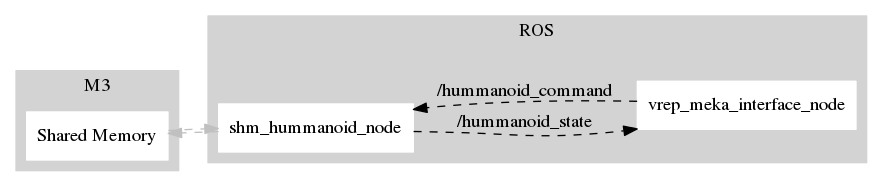
\includegraphics[width=1\linewidth]{figs/shm_arch}
    \caption{Arquitetura Controle C++}
    \label{fig:shm_arch}
\end{figure}

Todo o código relacionado ao controle do robô é disponibilizado pelo fabricante e compõe a biblioteca M3, implementada em Python e com interface em C++. A partir da análise do código foi possível observar alguns pontos importantes que contribuem para ineficiência dos controladores implementado anteriormente:

\begin{itemize}
    \item Apenas controle por posição de juntas está implementado em C++
    \item A taxa de atualização da memória compartilhada é de $100 Hz$
\end{itemize}

Dentro do programa de interface com o ROS foi possível observar alguns pontos importantes que contribuem para ineficiência dos controladores controladores de posição com e sem compensação da gravidade. Os valores de velocidade e torque informados para o controle são completamente ignorados. Além disto a taxa de envio da informação obtida pelo ROS para a memória compartilhada é de apenas $100Hz$ definidos \textit{hardcode}. Foi feito um teste para alterar este valor para $1KHz$ porém o robô ficou completamente instável. De movo que novos testes não foram repetidos para evitar danos ao robô.

Este valor é bem próximo das taxas de amostragem de $8 ms$ ($125 hz$) e $20 ms$ ($50 Hz$) dos controladores implementados em C++ obtidas para os melhores resultados em \cite{nobody} obtidos por Marco Pereira. Sendo estes valores definidos pelo tempo mínimo necessário para efetuar todos os cálculos relacionados ao controladores cinemáticos implementados usando quatérnions duais.

\section{Estudo Controladores Meka}

\subsection{API Python}

Para avaliar os controladores de junta de baixo nível foi utilizado a API em Python e a partir dai foram feitos vários teste a partir de comandos de posição para as juntas. A estrutura para envio dos comandos para o robô é diferente, de modo que alguns testes relacionados a comunicação também foram necessários. Estão estão disponíveis os seguintes controladores, ordenados do de mais alto nível para o de mais baixo nível:

\begin{itemize}
    \item Posição
    \item Velocidade
    \item Torque
    \item PWM
\end{itemize}

Os modos de controle de posição estão ainda disponíveis com e sem controle de compensação da gravidade.

\subsubsection{Avaliação do Atraso de Comunicação}

A comunicação com o robô é feita através de uma memória compartilhada. Assim, o primeiro experimento foi levantar o tempo gasto pela instrução \textit{proxy.step()} que atualiza esta memória pegando as medidas dos sensores e informando os comandos para os controladores. Este teste foi feito através avaliando o intervalo de tempo entre cada chamada após sucessivas interações tendo como resultado o valor médio de 16ms entre cada chamada indicando que a frequência máxima possível para um controlador implementado com base na API é de $f = 1/16ms = 62.5Hz$. Isto, obviamente, desconsiderando qualquer tempo extra gasto com as operações realizadas pelo próprio controlador.

\subsubsection{Avaliação do Acumulo do Erro}

Para verificar o acumulo do erro após sucessivas interações foi feito o teste de fechar a malha com braço na posição de repouso. Isto é, controle deveria ler os dados atuais do sensores e passar diretamente para o robô na expectativa de que o robô ficasse parado. No entanto foi observado que o braço começou a subir lentamente, indicando valores cada vez maiores para os ângulos medidos e uma distância cada vez maior da posição de origem.

Por outro ao ser enviado a mesma posição de referência suscetivamente, o braço desloca até o ponto desejado e permanece parado, mostrando que o controle para um referência em degrau é estável. O que viabilizou os testes de identificação a partir do uso de uma entrada em Degrau.

\subsubsection{Entrada em rampa}

Foram então feitos testes para um referência em rampa. Como se trata de um controle feito de maneira discreta, foram passados valores de ângulos em sequência incrementados por um valor contante e separados por um pequeno tempo de espera emulando uma entrada em rampa porém discretizada no tempo.

Para estudo da velocidade de resposta do controlador, o valor incrementado entre um ângulo e outro foi mantido enquanto o intervalo de tempo era ajustado. Neste experimento foi observado que para intervalos muito pequenos de tempo o robô não consegue acompanhar mantendo uma velocidade constante. Em tais casos a velocidade é mantida aproximadamente constante e com o acúmulo do erro ocorre saltos periódicos para compensar o atraso em relação a referência. Este fato decorre da interação entre o controlador de posição das juntas e o controlador de torque. O erro acumulado é corrigido com a passagem de um torque mais alto produzindo um salto na posição, seguido de uma leve oscilação para compensar o efeito da inercia.

% Repete testes ?

\subsubsection{Resposta ao Degrau}

Feito uma avaliação preliminar para o experimento de identificação da planta foi aplicado um degrau para cada uma das juntas individualmente com registro dos dados. Este teste foi definido a partir dos seguintes passos:

\begin{enumerate}
    \item Começa com a junta na posição $0$ graus
    \item Envia o comando para ir para posição $45$ graus
    \item Mantém a referência da posição em $45$ graus por $2s$
    \item Envia o comando para ir para posição $0$ graus
    \item Mantém a referência da posição em $0$ graus por $2s$
\end{enumerate}

Para a API em Python estes passos foram executados 3 vezes para cada uma das juntas. Um experimento semelhante foi efetuado a partir de um programa em C++ baseado no código elaborado em trabalhos anteriores. Para ambos casos a saída dos sensores foi registrada a partir do ROS a partir do programa rosbag e somente para os testes feitos em C++ foram também registradas os mensagens de controle. Uma vez que os comandos passados via API são enviados diretamente para o serializador de mensagens sem passar pelo ROS e portanto foram utilizados apenas para uma avaliação preliminar do comportamento dos controladores de junta. Mais detalhes do experimento em C++ na seção \ref{subsec:stepcpp}. 

% Qual foi a diferença dos dois para os mesmo parâmetros?
% Por que não foram avaliados outros ângulos?

\subsubsection{Controle de Posição sem Compensação da Gravidade}

O controle de posição sem o uso de compensação da gravidade foi avaliado em estudo e não foi possível atingir a posição desejada de 45 graus partido do zero em nenhuma das juntas. Na maioria dos caso o braço movia apenas 10 graus. O que explicita o fato do impacto de toda a estratégia de compensação da gravidade ser feita por software, diferente de outras plataformas como o Baxter em que esta é feita de forma mecânica \cite{nobody}.

Para tal é tomado a posição de referência passada

\subsubsection{Controle de Velocidade}

Foi feito apenas um ensaio utilizando o controle de velocidade disponível na API em Python. No entanto ao ser definido velocidade zero a braço robótico ficou completamente rígido e passou a ignorar comandos para outros valores de referência de velocidade. O que demonstrou um esforço grande sendo feito pelo controle de torque e pelos motores. Somente quando foi alterado o modo de controle para posição que o braço voltou a mover normalmente. Para evitar qualquer dano a plataforma, não foram feitos outros testes neste modo de operação.

% Teria como controlar a velocidade diretamente ?

\subsubsection{Controle de Torque}

O controle de torque está disponível em dois modos: com e sem compensação da gravidade. Na estratégia sem compensação da gravidade, o valor de referência de torque é passado diretamente a controlador das juntas.

% Por que não foi avaliado o controle de torque?

\section{Estudo Controladores Cinemáticos}

Em C++ não estão disponíveis todos os modos de operação para o uso a partir do ROS, embora ao final a mensagem seja serializada e passada para os mesmos programas. No nó $shm\_hummanoid$ está implementado somente o controle por posição com e sem compensação da gravidade. Em decorrência disto, foi analisado somente o controlador de posição com compensação da gravidade por ter sido o utilizado em trabalhos anteriores. Os tempos foram obtidos a partir do $ros::time$ e registrado nas mensagens como \textit{timestamp}. Foi necessário alterar o código do $vrep\_meka\_interface$ para incluir o \textit{timestamp} na mensagem para permitir a análise dos dados registrados via \textit{rosbag}. Em razão disto, alguns dos experimentos anteriores não foram incluídos no estudo do tempo de resposta por conta de inexistir um referencial de tempo comum para as mensagens do tópico $/hummanoid\_state$ e $/hummanoid\_command$.

\subsection{Controle de Posição de Juntas}\label{subsec:stepcpp}

Feito uma avaliar a resposta do controlador em C++ foi aplicado um degrau para cada uma das juntas individualmente com registro dos dados. Este teste foi definido a partir dos seguintes passos:

\begin{enumerate}
    \item Começa com a junta na posição $0$ rad
    \item Envia o comando para ir para posição $1$ rad
    \item Mantém a referência da posição em $1$ rad por $4s$
    \item Envia o comando para ir para posição $0$ rad
    \item Mantém a referência da posição em $1$ rad por $4s$
\end{enumerate}

Estes passos foram repetidos, ajustando-se os os parâmetros de rigidez e velocidade máxima do controlador. A velocidade máxima de cada junta pode ser ajusta para um valor entre $0$ e $1$, de igual forma a rigidez do braço gerada pelo controlador também pode ser ajustada entre $0$ e $1$. Valores maiores que 1 foram testados porém não houve mudança significativa em relação a comportamento com valor $1$. Muito embora em trabalhos anteriores na plataforma fosse usado $rigidez = 5$. Vale reforçar que estes são parâmetros usados pelos controladores no PC ( posição e compensação da gravidade ) de forma que não é possível obter diretamente os parâmetros de rigidez e velocidade máxima pela resposta do estado atual fornecida por \textit{/hummanoid\_state}.

Já no experimento feito de referência mostrado na \ref{fig:jointIdentification_exp2v100v50}, pode-se notar que existe um atraso de cerca de $20ms$ entre o comando e o recebimento do sinal de resposta do atuador no tópico. Também percebe-se um erro grande em regime permanente das juntas do pulso ($5$ e $6$). Percebe-se uma longa rampa indicando aonde o controle da posição passou a atuar como um controle tudo ou nada passando a velocidade máxima possível. Curiosamente, embora sejam motores distintos em cada uma das juntas com diferentes limites de velocidade a resposta do controlador é indica uma velocidade bem parecida de atuação nesta configuração.

\begin{figure}[H]
    \centering
    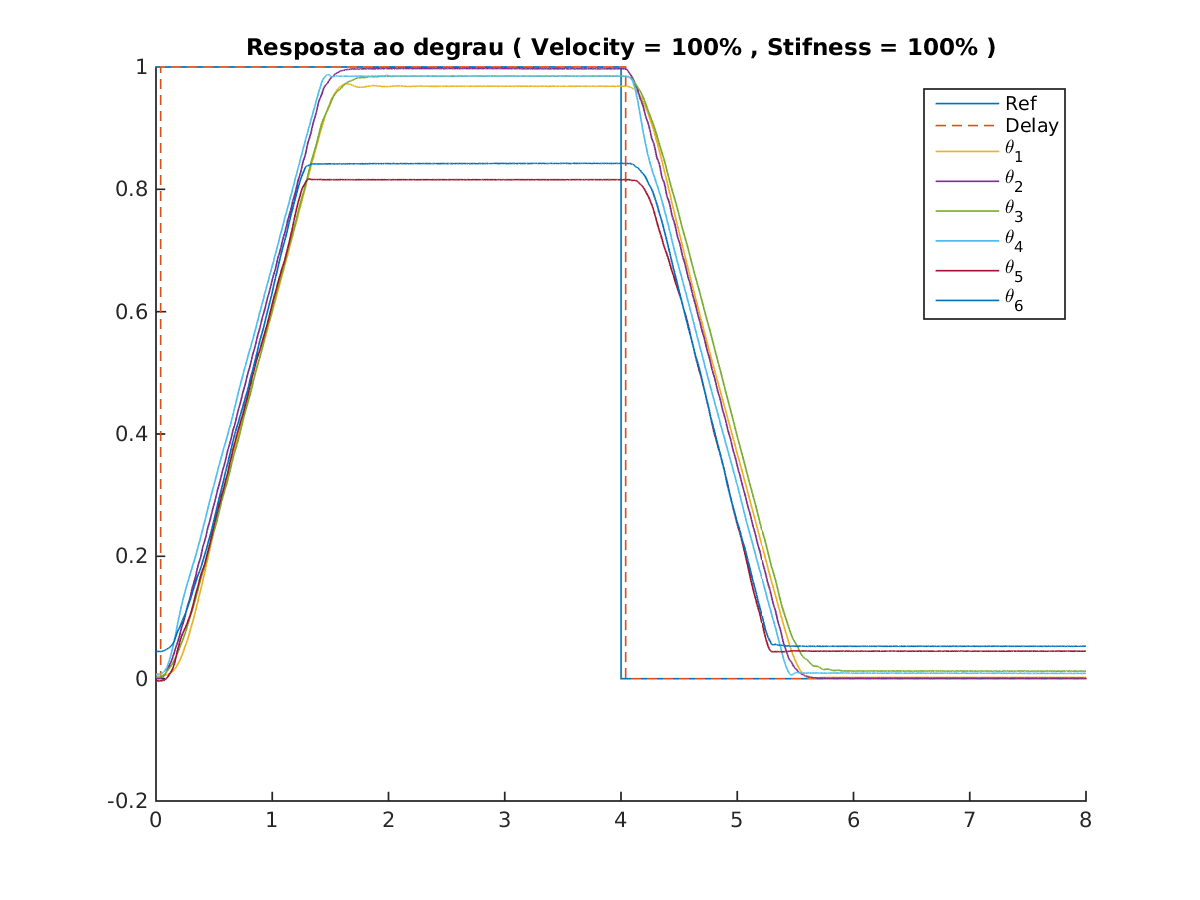
\includegraphics[width=0.6\linewidth]{tex/figs/jointIdentification_exp1v100v100.png}
    \caption{Resposta a um degrau de entrada com Velocidade = 1 e Rigidez = 1}
    \label{fig:jointIdentification_exp1v100v100}
\end{figure}

Pela figura \ref{fig:jointIdentification_exp2v100v50} observa-se que a variação da rigidez do controlador implica em um erro maior em regime permanente nas juntas. O controlador converge em um tempo próximo mas notadamente aumenta o erro das juntas do pulso. Este fato também é percebido no código de demonstração no ajuste da rigidez. Pois ao mudar o valor, mantida a mesma referência de posição o pulso desloca significativamente de posição.

\begin{figure}[H]
    \centering
    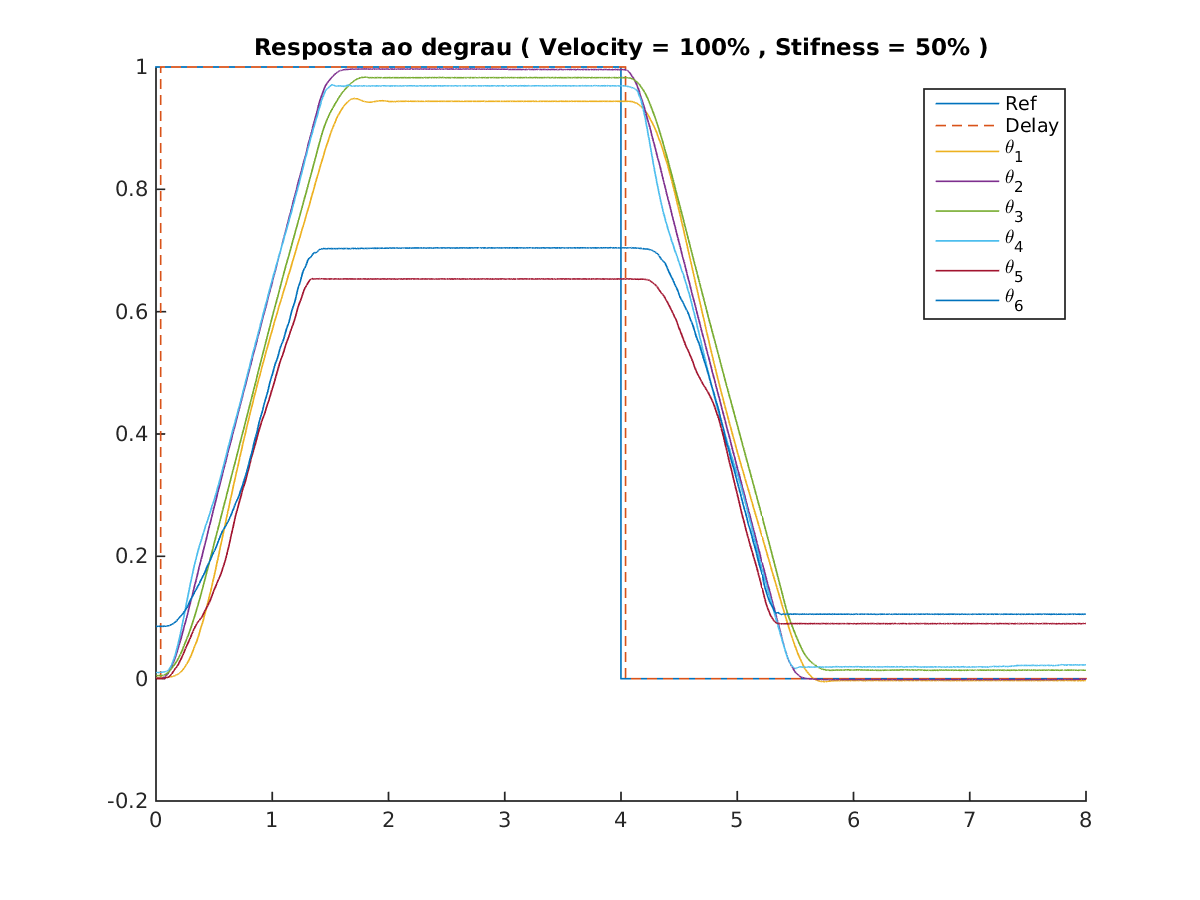
\includegraphics[width=0.6\linewidth]{tex/figs/jointIdentification_exp2v100v50.png}
    \caption{Resposta a um degrau de entrada com Velocidade = 1 e Rigidez = 0.5}
    \label{fig:jointIdentification_exp2v100v50}
\end{figure}

Como esperado, no terceiro experimento ao se alterar a velocidade para $70\%$ o tempo necessário para cada uma das juntas atingir a posição aumentou, tendo em vista a fase em que o controlador utiliza a velocidade máxima permitida, o erro em regime permanente para cada um permanece com pouca alteração. No entanto é percebido que a inclinação da curva durante as fase de controle entre o tempo $t=1s$ e $2s$ com a velocidade máxima muda de forma diferente para cada uma duas juntas. Estes dados encontram-se na figura \ref{fig:jointIdentification_exp3v70v100}.

\begin{figure}[H]
    \centering
    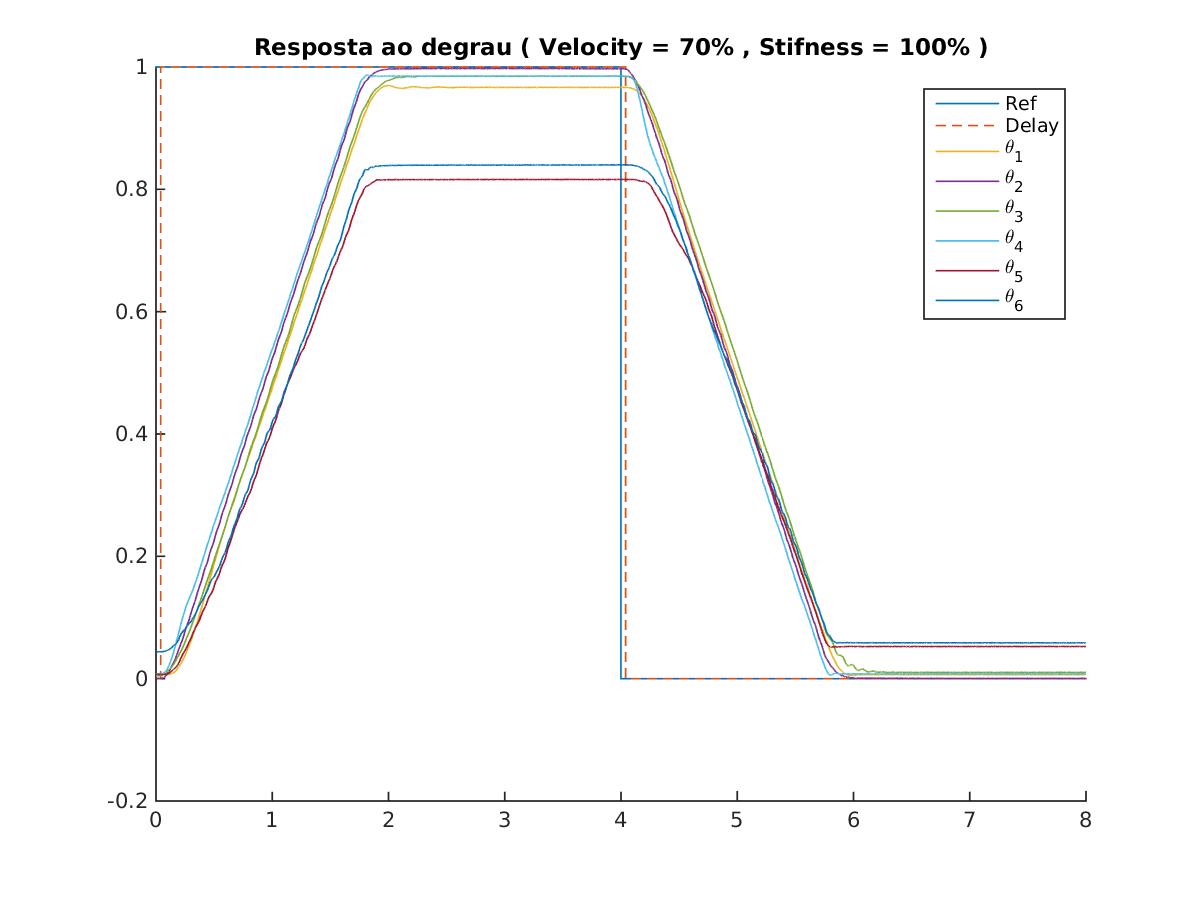
\includegraphics[width=0.6\linewidth]{tex/figs/jointIdentification_exp3v70v100.png}
    \caption{Resposta a um degrau de entrada com Velocidade = 0.7 e Rigidez = 1}
    \label{fig:jointIdentification_exp3v70v100}
\end{figure}

No 3 experimentos o atraso obtido foi próximo de $20ms$. Este valor é próximo dos valores de intervalo de tempo obtidos para os melhores resultados dos controladores implementados em \ref{nocite}. Notadamente, quando o controlador opera com frequências maiores, haverá o impacto do atraso da comunicação passa a ser mais significativo levando a instabilidade caso este não seja considerado no dinâmica implementada.

% Comentar sobre o varição do intervalo de tempo medido da entre os comandos enviados para a \hummanoid_command

Tomando-se o diferença entre o valor passado de referência e o valor alcançado tempo foram obtidos os erro em regime permanente, registrados na tabela \ref{tab:jointIdentification_errortable}.

\begin{table}[H]
    \centering
    $$\begin{array}{cc|ccccccc}
         \hline
         V & S & \theta_0 & \theta_1 & \theta_2 & \theta_3 & \theta_4 & \theta_5 & \theta_6\\
         \hline
         -Inf & 0.031544 & 0.0025193 & 0.014824 & 0.014865 & 0.18436 & 0.15769\\
-Inf & 0.056071 & 0.0036188 & 0.017413 & 0.031003 & 0.34662 & 0.29566\\
-Inf & 0.033305 & 0.0026167 & 0.015199 & 0.014783 & 0.18398 & 0.16037\\
-Inf & 0.056453 & 0.0035564 & 0.017352 & 0.03028 & 0.32879 & 0.28538\\

         \hline
    \end{array}$$
    \caption{Error Percentual para diferentes valores de velocidade ($V$) e rigidez ($S$)}
    \label{tab:jointIdentification_errortable}
\end{table}

\begin{table}[H]
    \centering
    $$\begin{array}{cc|ccccccc}
         \hline
         V & S & \theta_0 & \theta_1 & \theta_2 & \theta_3 & \theta_4 & \theta_5 & \theta_6\\
         \hline
         0 & 1.0041 & 1.0001 & 1.0002 & 1.0025 & 1.0016 & 0\\
0 & 1.0049 & 1.0004 & 1.0008 & 1.0019 & 1.0007 & 0\\
0 & 1.003 & 1.0002 & 1.0004 & 1.0016 & 0 & 0\\
0 & 1.005 & 1.0004 & 1.0009 & 1.0026 & 0 & 0\\

         \hline
    \end{array}$$
    \caption{Percentual Overshot para diferentes valores de velocidade ($V$) e rigidez ($S$)}
    \label{tab:jointIdentification_overshottable}
\end{table}

\begin{table}[H]
    \centering
    $$\begin{array}{cc|ccccccc}
         \hline
         V & S & \theta_0 & \theta_1 & \theta_2 & \theta_3 & \theta_4 & \theta_5 & \theta_6\\
         \hline
         1.00 & 1.00 & 0.001841 & 0.96846 & 0.99748 & 0.98518 & 0.98513 & 0.81564 & 0.84231\\
1.00 & 0.50 & 0.003698 & 0.94393 & 0.99638 & 0.98259 & 0.969 & 0.65338 & 0.70434\\
0.70 & 1.00 & 0.0020654 & 0.9667 & 0.99738 & 0.9848 & 0.98522 & 0.81602 & 0.83963\\
1.00 & 0.50 & 0.0047216 & 0.94355 & 0.99644 & 0.98265 & 0.96972 & 0.67121 & 0.71462\\

         \hline
    \end{array}$$
    \caption{Valor em regime permanente para diferentes valores de velocidade ($V$) e rigidez ($S$)}
    \label{tab:jointIdentification_steadstatetable}
\end{table}

% Acrescentar Tempo de Resposta 

\subsection{Controladores Cinemáticos usando Quatérnions Duais}

% Obter dt em /hummanoid_state e /hummanoid_command para cada um dos casos
% Experimento MoveUP

Os controladores de posição do efetuador foram avaliado a partir da estratégia de discretização dos pontos e frequência de amostragem. Para tal foi reduzido o número de ponto e trajetória foi simplificada para apenas um deslocamento em linha reta de 10cm na vertical. Para primeira análise foi utilizado os controladores implementados anteriormente e foram feitos os seguintes testes:

\begin{enumerate}
    \item Trajetória dividida em $100$ pontos, intervalo de $8 ms$
    \item Trajetória dividida em $100$ pontos, intervalo de $100 ms$
    \item Trajetória dividida em $1000$ pontos, intervalo de $8 ms$
\end{enumerate}

Foi observado que o robô leva um tempo até começar a mexer e um tempo até o controle estabilizar. De modo que está sempre atrasado em relação a referência. Para o período $8 ms$ foram necessárias $25$ interações até o robô começar a se mover, com o período de $100 ms$ o robô começo a se mover já na segunda interação sugerindo um atraso na comunicação de $200 ms$ entre o tempo que o comando é passado via ROS e o tempo que o robô executa o comando.

% Gráficos ?

% Saltos a cada 300 ms

\section{Estudo sobre não linearidades}

% Acrescentar simulação no simulink pControlSaturation
% - Comparativo da resposta para o mesmo ganho em um sistema de primeira ordem ( com delay e saturação )
% - Verificar necessidade de mudar a ordem e puxar a seção para antes

Uma vez que os modelos usados para o controle são lineares, a existência de comportamentos não lineares representam perturbações e podem gerar erros ou até instabilidade no controle caso não consideradas. Em razão disto uma atenção especial foi dada a este aspecto visando identificar a contribuição da perca de desempenho. A grande dificuldade é podem ocorrem em qualquer uma das partes do sistema de controle gerando um acumulo do efeito com o aumento da quantidade de camadas em cascata.

\subsection{Saturação do Atuador}

O efeito de saturação do atuador ocorre quando é solicitado uma ação de torque ou velocidade acima do que o atuador permite. Em diversos sistemas isto é limitado através de algum dispositivo de proteção evitando danificar o atuador. Do lado do controle, este é percebido como uma resposta mais lenta que o esperado para aquele determinado ganho em simulação podendo levar a instabilidade no controle do sistema real.

Como o controle da posição é feito em colaboração pela ação de cada uma das juntas, este problema é mascarado na métrica do erro de posição. Como a contribuição de cada junta em manipulador não cartesiano muda de acordo com a posição, o atraso devido a saturação pode fazer com que o robô tenha um erro maior para determinadas posições no decorrer da trajetória que outras. Outro efeito é a saturação de um motor levar a um uso maior dos outro motores na tentativa de compensar o erro acumulado. Como são utilizados diferentes motores para cada uma das juntas, conferindo limitações especificas na atuação, em particular na velocidades máximas que cada junta pode atingir. Por conta disto, é percebido um maior uso das juntas com velocidade máxima maior para compensar o erro acumulado pela juntas com velocidade máxima menor, quando o controle começa solicitar uma velocidade maior que a permitida pelos outros motores. Em particular no Meka, este fenômeno leva a um uso maior das juntas do ombro para corrigir orientação ao acumulado pela saturação das juntas do pulso.

Em um manipulador robótico composto por juntas rotacionais, a tarefa de deslocamento no espaço é distribuída entre todas as juntas ao longo de praticamente toda a região do espaço de trabalho. O deslocamento de cada junta produz um arco que inevitavelmente gera movimentação em pelo menos duas direções no espaço e uma rotação. Desta forma o tarefa de atingir uma posição e orientação no espaço é distribuída por várias juntas, permitindo um esforço menor em um determinado atuador. No entanto, em particular para um braço antropomórfico a orientação é resolvida de forma conjunta pelo pulso e pelo ombro gerando um amplo espaço nulo a permitindo para uma mesma posição do pulso, diversas posições para o cotovelo.

Tais relações geométricas indicam que a tarefa de manter uma orientação possui uma relação com o movimento necessário pelas juntas notadamente diferente da tarefa de manter uma posição. De forma a permitir separar a complacência da posição ou da orientação conforme necessário para a tarefa. Ao se utilizar a representação cinemática por Quatérnions Duais tanto a referência da posição como a da orientação estão acopladas. Um bom controlador por outro lado necessita de uma rápida resposta a uma perturbação, gerando uma rigidez maior ao invés de uma complacência. Como para os experimentos em questão a orientação de referência era mantida como a orientação inicial do robô, parte do esforço de controle era direcionado em manter a orientação. O que gerava uma pertubação na posição. Este problema em composição com diferença de velocidade dos atuadores do pulso e da ombro fazia com que uma perturbação na orientação percebida no pulso provoca-se uma movimentação juntas do ombro e por consequência uma movimentação da posição do cotovelo. O que gerava uma aproximação do cotovelo para a base provocando em cascata uma maior chance colisão do braço com o tronco e uma dificuldade em manter a estabilidade as referências do controle através da cinemática diferencial. Pois o robô se aproximava do limite da junta e de regiões com bloqueio de movimento.

As consequências deste fenômeno foram atenuadas pelos primeiro trabalhos com o acréscimo de uma espuma de proteção no tronco do robô, minimizando o risco de dano. Em \cite{nobody} foi resolvida pelo Marcos Pereira pela escolha de posições iniciais com o cotovelo distante do tronco e operando em uma região limitada por um plano paralelo a frente do robô. Em \cite{nobody}, Rafael Koji, no capítulo 3, página 33, apresenta como solução a separação do acoplamento do controle das 2 juntas do pulso ($j5$ e $j6$) com a redução do modelo cinemático do manipulador para 5 juntas apenas. O que permitindo o controle de posição em malha fechada com 5 graus de liberdade e a orientação em malha aberta pelas juntas do pulso, reduzindo as instabilidades. Em experimento disponível no YouTube \footnote{https://www.youtube.com/watch?v=bU7Ocphhifg} Luís Sentis demonstra a utilização de campos potenciais como forma de manter a postura do robô e evitar a colisão enquanto permite a priorização do controle complacente em uma das 3 direções $X$, $Y$ e $Z$ a partir da arquitetura implementada em \cite{sentis2007synthesis} no Meka.

% aqui entra o kung-fu 

% Citar o trabalho da UT com campo de potenciais

% Fenômeno Harakiri: O cotovelo do meka vai se aproximando do tronco com o passar do tempo, o robô move bruscamente com pertubações na orientação a partir da posição de referência usada nos trabalhos do Koji e do Marcos

% Montar experimentos Harakiri 2DOF, Harakiri Meka em simulação no Matlab, Harakiri Meka real
% Estudo do erro por junta ao invés de por posição -> Pontuar necessidade introduzir novas métricas

\subsection{Atraso da Comunicação}

Dado a existência de várias camadas entre o controle cinemático e o atuador de fato, existe um atraso na comunicação que influência na dinâmica do sistema. O controlador cinemático interagem com o ROS que por sua vez interage com uma memória compartilhada que é atualizada com um frequência de $1 KHz$. Para avalia o atraso foi feito a medida a partir do ensaio em degrau, entre o tempo de envio do comando de controle no tópico $/humanoid_control$ e o primeiro instante em que a posição da junta atinge um valor diferente de zero na leitura do valor correspondente no tópico $/humanoid_state$. Uma vez que existe um pouco de ruído na leitura da posição, foi considerado a valor de referência $\Delta\theta_0 = 0.1 rad = 5^\circ$.

% Resultados

\subsection{Controle Virtual de Rigidez}

% Comparar com primeiras implementações de SEA

Com base no controle do torque e o uso de sensores de posição pode se emular o comportamento de uma mola com rigidez variável através de um controlador. Esta estratégia é denominada mola virtual e permite conferir o controle de força com precisão sem a necessidade de ajustar fisicamente algum elemento elástico.

% Diagrama SEA Virtual